\documentclass[11pt,a4paper]{report}

\usepackage[a4paper, margin=1in]{geometry}
\usepackage{polski}
\usepackage[utf8]{inputenc}
\usepackage{indentfirst}
\usepackage{hyperref}
\usepackage{tikz}
\usepackage{graphicx}

\graphicspath{ {./images/} }

\usetikzlibrary{positioning}
\usetikzlibrary{calc}

\def\console #1{\begingroup\fontfamily{qcr}\selectfont#1\endgroup}
\newenvironment{multiconsole}{\begingroup\fontfamily{qcr}\selectfont}{\endgroup}



\title{\Huge JavaGridGraph - Dokumentacja}
\author{Skoczek Mateusz, Jędrzejewski Sebastian}
\date{\today}



\begin{document}
    \maketitle
        




    \begin{abstract}
        Dokument zawiera specyfikację funkcjonalną i implementacyjną dotyczącą projektu \textsl{JavaGridGraph} oraz opis testów programu.
    \end{abstract}





    \tableofcontents
    \thispagestyle{empty}





    \newpage
    \chapter{Specyfikacja funkcjonalna}




    \newpage
    \section{Cel projektu}

    Program \textbf{JavaGridGraph} ma na celu wygenerowanie grafu siatkowego o podanych paramentrach oraz zapisanie go do pliku lub wczytanie grafu z pliku oraz sprawdzenie wybranych jego parametrów. Program posiada interfejs graficzny. Grafy są przedstawiane w plikach w postaci listy sąsiedztwa.




    \newpage
    \section{Opis funkcji}

    Program oferuje dwie główne funkcje: generowanie grafu oraz sprawdzanie grafu.

    \vspace{4em}

    Program pozwala wygenerować graf o:
    
    \begin{itemize}
        \item określonej wysokości (ilości wierszy)
        \item określonej szerokości (ilości kolumn)
        \item określonej minimalnej i maksymalnej wadze krawędzi
        \item określonej minimalnej i maksymalnej ilości krawędzi wychodzących z pojedyńczego wierzchołka
        \item stałym ziarnie generatora liczb losowych
    \end{itemize}

    Program umożliwia zapis wygenerowanego grafu do pliku oraz/lub wczytanie grafu do sprawdzenia.
    
    \vspace{4em}

    W ramach funkcji sprawdzania grafu, program pozwala na sprawdzenie następujących parametrów wczytanego grafu:

    \begin{itemize}
        \item spójność grafu
        \item najkrótsze ścieżki od wybranego wierzchołka $A$ do wybranych wierzchołków $B_n$
    \end{itemize}




    \newpage
    \section{Opis interfejsu programu}

    \subsection{Widok startowy}

    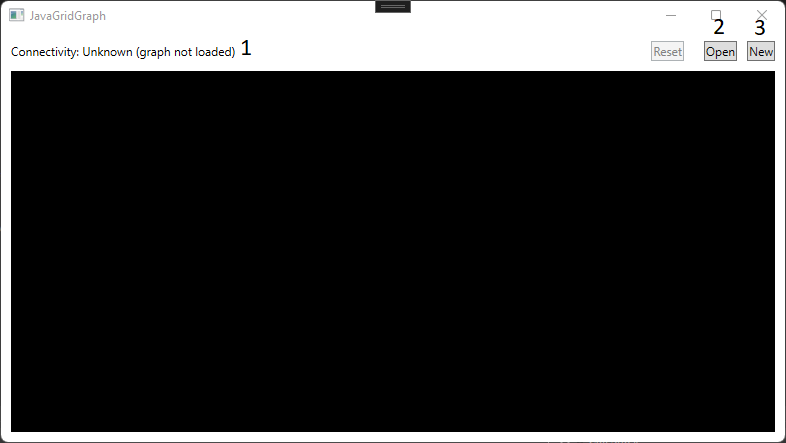
\includegraphics[width=\textwidth]{view1.png}

    \begin{enumerate}
        \item Wynik sprawdzenia spójności grafu. W przypadku gdy graf nie został wczytany, zostanie pokazana informacja o tym że graf nie został wczytany.
        \item Przycisk "Open" otwiera systemowe okno wyboru pliku w celu wybrania pliku zawierającego graf
        \item Przycisk "New" otwiera okno generowania grafu. Więcej informacji w punkcie "Okno generowania grafu".
    \end{enumerate}
\end{document}